\PassOptionsToPackage{dvipsnames}{xcolor}
\documentclass{beamer}
\usepackage{xcolor}
\usepackage{pgfpages}

\usepackage[style=authortitle]{biblatex}

\setbeameroption{show notes on second screen}

\usepackage[utf8]{inputenc}
\usepackage[T1]{fontenc}
\usepackage{lmodern}
\usepackage{fontawesome}

\usepackage{minted}

\usepackage{listings}

\usepackage[american]{babel}

\usepackage{
    amsmath,
    amsfonts,
    amssymb
}

\usepackage[os=win]{menukeys}

\usetheme{UOS}

\graphicspath{{img/}}

% use this with \begin{pythoncode} ... \end{pythoncode}
\newminted{python}{linenos=false}

\newminted[outputcode]{text}{linenos=false}

% this gets rid of red boxes around syntax errors in minted
\AtBeginEnvironment{minted}{%
  \renewcommand{\fcolorbox}[4][]{#4}}

% removes the prefix "Figure 1:" in figure captions
\setbeamertemplate{caption}{\raggedright\insertcaption\par}


\begin{document}

\title[Introduction]{Week 3: Control Structures}
\subtitle{Basic Programming in Python}

\author[kgross, mpoemsl, sselbach]{Katharina Groß, Martin Pömsl, Sören Selbach}

% change to date of actual lecture
\date{\today}

\begin{frame}[plain]
    \titlepage
\end{frame}

\begin{frame}
    \tableofcontents
\end{frame}

\section{Recap}

\subsection{Booleans}

\begin{frame}{Recap: Booleans}

    \begin{itemize}
        \item Boolean variables are either \texttt{True} or \texttt{False}
        \item Booleans are the result of \textit{comparisons:}

        \begin{itemize}
            \item \texttt{41 > 42} results in \texttt{False}
            \item \texttt{"basicpython" == "basic" + "python"} results in \texttt{True}
        \end{itemize}

        \item There are also operators which act directly on Booleans:

        \begin{itemize}
            \item \textbf{\texttt{not x}} is \texttt{True} if \texttt{x} is \texttt{False} and vice versa
            \item \textbf{\texttt{x and y}} is \texttt{True} if both \texttt{x} and \texttt{y} are \texttt{True}
            \item \textbf{\texttt{x or y}} is \texttt{True} if at either \texttt{x} or \texttt{y} is \texttt{True}, \textbf{or both}
        \end{itemize}

    \end{itemize}

    \note{
        \begin{tabular}{| r | r |}
            \hline
            \textbf{\texttt{x}} & \textbf{\texttt{not x}} \\
            \hline
            \color{Red}{\texttt{False}} & \color{Green}{\texttt{True}} \\
            \color{Green}{\texttt{True}} & \color{Red}{\texttt{False}} \\
            \hline
        \end{tabular}

        \vspace{1em}

        \begin{tabular}{| r r | r |}
            \hline
            \textbf{\texttt{x}} & \textbf{\texttt{y}} & \textbf{\texttt{x and y}} \\
            \hline
            \color{Red}{\texttt{False}} & \color{Red}{\texttt{False}} & \color{Red}{\texttt{False}} \\
            \color{Red}{\texttt{False}} & \color{Green}{\texttt{True}} & \color{Red}{\texttt{False}} \\
            \color{Green}{\texttt{True}} & \color{Red}{\texttt{False}} & \color{Red}{\texttt{False}} \\
            \color{Green}{\texttt{True}} & \color{Green}{\texttt{True}} & \color{Green}{\texttt{True}} \\
            \hline
        \end{tabular}

        \vspace{1em}

        \begin{tabular}{| r r | r |}
            \hline
            \textbf{\texttt{x}} & \textbf{\texttt{y}} & \textbf{\texttt{x or y}} \\
            \hline
            \color{Red}{\texttt{False}} & \color{Red}{\texttt{False}} & \color{Red}{\texttt{False}} \\
            \color{Red}{\texttt{False}} & \color{Green}{\texttt{True}} & \color{Green}{\texttt{True}} \\
            \color{Green}{\texttt{True}} & \color{Red}{\texttt{False}} & \color{Green}{\texttt{True}} \\
            \color{Green}{\texttt{True}} & \color{Green}{\texttt{True}} & \color{Green}{\texttt{True}} \\
            \hline
        \end{tabular}
    }

\end{frame}

\subsection{If-Statements}

\begin{frame}[fragile]{Recap: \texttt{if}-statements}

    \begin{block}{}
        \texttt{if}-statements can be used to direct the \textbf{flow} of the program
    \end{block}

    \begin{pythoncode}
        if <condition>:
            <do this if condition is True>
        else:
            <do this otherwise>
     \end{pythoncode}

     \begin{itemize}
         \item \textbf{\texttt{<condition>}} must be some expression that results in a Boolean
         \item if it is \textbf{\texttt{True}}, the code in the block after the \texttt{if} line is executed
         \item a \textbf{code block} are multiple consecutive lines that have the same \textbf{indentation}
     \end{itemize}

     \note{
        \begin{itemize}
            \item ... and if \texttt{<condition>} is \texttt{False}, the code in the \texttt{else}-block is executed
            \item in other languages like C or Java, code blocks are designated by \texttt{\{\}}.
        \end{itemize}
     }

\end{frame}

\begin{frame}[fragile]{\texttt{elif}}

    \begin{block}{}
        \textbf{\texttt{elif}} statements (short for \texttt{else if}) allow to check for an additional condition if the first one was \texttt{False}
    \end{block}

    \begin{pythoncode}
        if <condition 1>:
            <do this if condition 1 is True>

        elif <condition 2>:
            <do this if condition 2 is True>

        else:
            <do this otherwise>
    \end{pythoncode}

\end{frame}

\begin{frame}[fragile]{\texttt{elif}: Examples}

    \begin{columns}[totalwidth = \textwidth, T]

    \begin{column}{0.5\textwidth}

        \begin{pythoncode}
n = 42

if n > 100:
    print("if")

elif n > 20:
    print("elif")

else:
    print("else")
        \end{pythoncode}

        \pause
        \vspace{1em}

        \textbf{Output:} \texttt{elif}

    \end{column}

    \pause

    \begin{column}{0.5\textwidth}

        \begin{pythoncode}
n = 42

if n > 10:
    print("if")

elif n > 20:
    print("elif")

else:
    print("else")
        \end{pythoncode}

        \pause
        \vspace{1em}

        \textbf{Output:} \texttt{if}

    \end{column}

    \end{columns}

\end{frame}

\section{Loops}

\begin{frame}[fragile]

    \begin{block}{Task}
        We want to know how often we can divide a number by 2 (integer division) until we get 0
    \end{block}

    \pause

    \begin{pythoncode}
        if n == 0:
            print("Can divide 0 times.")
        else:
            n = n // 2
            if n == 0:
                print("Can divide 1 time.")
            else:
                n = n // 2
                if n == 0:
                    print("Can divide 2 times.")
                else: # ...

    \end{pythoncode}

    \note{
        Counting how often we can divide a number is basically computing its \textit{logarithm}.

        \vspace{1em}

        \textbf{Approach using \texttt{if} statements:}

        First, we check if \texttt{n} is already \texttt{0}. If yes, we can safely say that we could divide 0 times until we got 0. If not, we divide \texttt{n} by 2 once, and check if it is \texttt{0} \textit{now}. If yes, we can safely say that we could divide 1 time until we got 0 - and so on.

        \vspace{1em}

        Obviously, that is a bad approach. What if we want to be able to deal with numbers that need to be divided, say, 100 times? Writing 100 nested \texttt{if} statements is definitely impractical.
    }

\end{frame}

\begin{frame}

    \centering
\includegraphics[width=0.7\textwidth]{03_Control_Structures/da7.jpg}

\end{frame}

\subsection{While-Loop}

\begin{frame}[fragile]{While-Loop}

    \begin{pythoncode}
        while <condition>:
            <code to be executed>
    \end{pythoncode}

    \begin{block}{}
        Just as with the \texttt{if}-statement, the \texttt{while}-loop checks if the condition is \texttt{True} and executes the code block associated with it accordingly. However, when it reaches the end of the block it \textbf{jumps back to the condition}. If it is still true, the \texttt{while}-loop will run again!
    \end{block}

\end{frame}

\begin{frame}[fragile]{While-Loop: Example}

    \begin{pythoncode}
    n = input("Enter a number: ")
    counter = 0

    while n > 0:
        n = n // 2
        counter = counter + 1

    print("Can divide " + str(counter) + " times.")
    \end{pythoncode}

\end{frame}

\begin{frame}{While-Loop: Example}

    \begin{exampleblock}{}
        \textbf{Input: \texttt{42}}
    \end{exampleblock}
    \vspace{-1em}

    \begin{columns}[totalwidth=\textwidth, t]

    \begin{column}{0.5\textwidth}

        \begin{center}

        \begin{tabular}{r r r}
            \textbf{\texttt{n}} & \textbf{\texttt{counter}} & \textbf{\texttt{n > 0}} \\
            \hline \hline
            \texttt{\color{red}{42}} & \texttt{-} & \texttt{True} \\
            \texttt{42} & \texttt{\color{red}{0}} & \texttt{True} \\
            \hline \hline
            \texttt{\color{red}{21}} & \texttt{0} & \texttt{True} \\
            \texttt{21} & \texttt{\color{red}{1}} & \texttt{True} \\
            \hline
            \texttt{\color{red}{10}} & \texttt{1} & \texttt{True} \\
            \texttt{10} & \texttt{\color{red}{2}} & \texttt{True} \\
            \hline
            \texttt{\color{red}{5}} & \texttt{2} & \texttt{True} \\
            \texttt{5} & \texttt{\color{red}{3}} & \texttt{True} \\
        \end{tabular}

        \end{center}

    \end{column}

    \begin{column}{0.5\textwidth}

        \begin{center}

        \begin{tabular}{r r r}
            \textbf{\texttt{n}} & \textbf{\texttt{counter}} & \textbf{\texttt{n > 0}} \\
            \hline \hline
            \texttt{\color{red}{2}} & \texttt{3} & \texttt{True} \\
            \texttt{2} & \texttt{\color{red}{4}} & \texttt{True} \\
            \hline
            \texttt{\color{red}{1}} & \texttt{4} & \texttt{True} \\
            \texttt{1} & \texttt{\color{red}{5}} & \texttt{True} \\
            \hline
            \texttt{\color{red}{0}} & \texttt{5} & \texttt{\color{red}{False}} \\
            \texttt{0} & \texttt{\color{red}{6}} & \texttt{False} \\
            \hline \hline
            \multicolumn{3}{c}{\texttt{End of program.}}
        \end{tabular}

        \end{center}

    \end{column}

    \end{columns}

\end{frame}

\begin{frame}[fragile]{While-Loop: Another Example}

    \begin{block}{Task}
        We want to list all the number from 1 to 100
    \end{block}

    \pause

    \begin{pythoncode}
    counter = 1

    while counter <= 100:
        print(counter)

        # equivalent to counter = counter + 1
        counter += 1
    \end{pythoncode}

    \pause
    \vspace{1em}

    \textbf{This time we know in advance how often our loop will run!}

    \note{
        \begin{itemize}
            \item Expressions like \texttt{x += 3}, at least on numbers, are equivalent to \texttt{x = x + 3}. They \textit{increment} a variable by a certain value. Such shorthands exist for other operators as well: \texttt{-=}, \texttt{*=}, \texttt{/=}, \texttt{**=} and \texttt{\%=}. No, there is no \texttt{i++} in Python.
        \end{itemize}
    }

\end{frame}

\subsection{For-Loop}

\begin{frame}[fragile]{For-Loop}

    \texttt{for}-loops make tasks like this more elegant

    \vspace{1em}

    \begin{pythoncode}
    for i in range(100):
        print(i + 1)
    \end{pythoncode}

    \pause
    \vspace{1em}

    \begin{itemize}
        \item \texttt{i} is just another variable (replacing \texttt{counter})
        \item \texttt{range(100)} "includes" all the numbers from 0 to 99
        \item ... which is why we need the \texttt{+ 1}
    \end{itemize}

    \note{
        You can interpret such a \texttt{for}-loop like this:

        \begin{itemize}
            \item Define a variable \texttt{i} and assign the first value from \texttt{0} to \texttt{99} to it (which is \texttt{0})
            \item Execute whatever is in the \texttt{for}-loop's code block
            \item Assign the \textbf{next} value from \texttt{0} to \texttt{99} to \texttt{i} (if there is no more value, the loop is over) and execute the code block again
        \end{itemize}

        \vspace{1em}

        There is much more to the \texttt{for}-loop than meets the eye. We will see some more ways to use it in this course, and there are even more that we will not cover.

        \vspace{1em}

        Usually whenever you can use a \texttt{for}-loop, you could also use a \texttt{while}-loop and vice versa, but one is usually more elegant than the other.
    }

\end{frame}

\begin{frame}[fragile]{Ways to use \texttt{range}}

    \begin{pythoncode}
    # all integers from 0 - 99
    range(100)

    # all integers from 50 - 99
    range(50, 100)

    # all integers from 50 - 99 in increments of 2
    # note that this does not actually include 99
    range(50, 100, 2)
    \end{pythoncode}

\end{frame}

\begin{frame}[fragile]{For-Loop: Another Example}

    \begin{block}{Task}
        We want to draw a square spiral using the turtle
    \end{block}

    \pause

    \begin{columns}[totalwidth=\textwidth]

    \begin{column}{0.5\textwidth}

    \vspace{-2em}

        \begin{pythoncode}
    from turtle import *

    for i in range(20):
        forward(10 * i)
        left(90)
        \end{pythoncode}

    \end{column}

    \begin{column}{0.5\textwidth}
        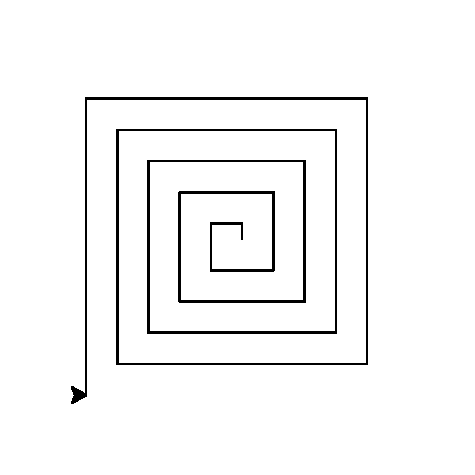
\includegraphics[width=\textwidth]{03_Control_Structures/spiral1}
    \end{column}

    \end{columns}

\end{frame}

\section{Functions}

\subsection{Re-Using Code}

\begin{frame}{}

    \vspace{0.5em}

    \begin{block}{Task}
        Now we would like to draw a spiral, do some stuff (like moving the turtle somewhere) and \textit{draw another spiral}
    \end{block}

    \vspace{-1em}

    
\includegraphics[width = \textwidth]{03_Control_Structures/spiral2}

\end{frame}

\begin{frame}[fragile]{Naive Approach}

    We could just copy and paste the code for the spiral:

    \begin{pythoncode}
        for i in range(20):
            forward(10 * i)
            left(90)

        # do some stuff here

        for i in range(20):
            forward(10 * i)
            left(90)
    \end{pythoncode}

    \pause

    \begin{alertblock}{\textbf{Problem}}
        This can get long and complicated before you know it!
    \end{alertblock}

    \note{
        Technically, a programming language with branches (i.e. \texttt{if}-statements) and repetitions (i.e. loops) is \textit{Turing complete}, meaning we can compute just about anything with it. Much of the stuff that we will learn next "only" makes Python more convenient to use, although that is probably the biggest understatement of this course.
    }

\end{frame}

\begin{frame}[fragile]{Functions}

    \vspace{-1em}

    \begin{block}{}
        Functions can be used to organize and re-use code
    \end{block}

    \vspace{1em}

    \begin{columns}[totalwidth=\textwidth]

    \begin{column}{0.5\textwidth}

        \vspace{-0.4em}

        \begin{pythoncode}
def draw_spiral():
    for i in range(20):
        forward(10 * i)
        left(90)

draw_spiral()
# do some stuff here
draw_spiral()
        \end{pythoncode}

    \end{column}

    \begin{column}{0.5\textwidth}

        \begin{alertblock}{}
            Here we \textbf{define} a function named \texttt{draw\_spiral} which contains our code for drawing a spiral
        \end{alertblock}

        \begin{alertblock}{}
            Here we \textbf{call} the function (twice) \textit{Only here is the function actually executed}
        \end{alertblock}

    \end{column}

    \end{columns}

\end{frame}

\subsection{Arguments}

\begin{frame}[fragile]{Passing Arguments}

    \begin{block}{Task}
        We want to let our \texttt{draw\_spiral} function have a variable number of loops
    \end{block}

    Arguments/parameters are a way of making a function \textbf{depend on a variable}

    \begin{pythoncode}
    def draw_spiral(loops):
        for i in range(4 * loops):
            forward(10 * i)
            left(90)

    draw_spiral(3)  # will draw a spiral with 3 loops
    draw_spiral(5)  # will draw a spiral with 5 loops
    \end{pythoncode}

    \note{
        Although "argument" and "parameter" are often used synonymously, there is a difference:

        \begin{itemize}
            \item \textit{Arguments} are what is used inside a \textbf{function call}, e.g. the string in \texttt{print("derp")}
            \item \textit{Parameters} are the variables inside a \textbf{function definition}
        \end{itemize}
    }

\end{frame}

\begin{frame}{Passing Arguments}

    \vspace{-1em}

    \begin{columns}[totalwidth = \textwidth]

    \begin{column}{0.5\textwidth}

        
\includegraphics[width = \textwidth]{03_Control_Structures/spiral3}
        \centering{\texttt{draw\_spiral(3)}}

    \end{column}

    \begin{column}{0.5\textwidth}

        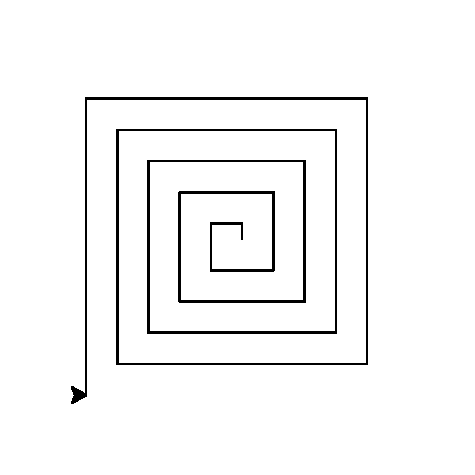
\includegraphics[width = \textwidth]{03_Control_Structures/spiral4}
        \centering{\texttt{draw\_spiral(5)}}

    \end{column}

    \end{columns}

\end{frame}

\begin{frame}[fragile]{Default Parameter Values}

    \begin{block}{}
        We can give parameters a \textbf{default value} which is assumed if no argument is given
    \end{block}

    \begin{pythoncode}
    def draw_spiral(loops = 5):
        for i in range(4 * loops):
            forward(10 * i)
            left(90)

    draw_spiral()   # will draw a spiral with 5 loops
    draw_spiral(3)  # this still works
    draw_spiral(loops = 42) # this works as well
    \end{pythoncode}

\end{frame}

\begin{frame}[fragile]{Another Example: Factorial}

    \begin{alertblock}{\textbf{Reminder: Factorial}}
        $$ n! = \prod_{i=1}^n i = 1 \cdot 2 \cdot 3 \cdot ... \cdot (n - 1) \cdot n $$
    \end{alertblock}

    \begin{pythoncode}
    def print_factorial(n):
        product = 1

        for i in range(1, n + 1):
            product *= i
            # equivalent to product = product * i

        print(product)
    \end{pythoncode}

    \note{
        \begin{itemize}
            \item As a rule of thumb, you should only print in functions that have "\texttt{print}" in their name (or "\texttt{output}" etc.). The same goes for drawing with the turtle.
        \end{itemize}
    }

\end{frame}


\subsection{Return Values}

\begin{frame}{Return Values}

    \begin{block}{}
        What if we need the result of a function later on in our program?
    \end{block}

    Simply printing it does not work as we have no (easy) way of recovering what was printed

    \pause
    \vspace{1em}

    \begin{alertblock}{\textbf{\texttt{return} statements}}
        \texttt{return} statements return a value from inside a function to the caller of the function. They make functions behave more like mathematical functions in that they "map" the arguments to a value.
    \end{alertblock}

    \note{
        \begin{itemize}
            \item We also cannot access the variable \texttt{product} from outside the function because it was \textit{defined inside} of it. This is called a \textbf{local} variable.
        \end{itemize}
    }

\end{frame}

\begin{frame}[fragile]{Return Values: Example}

    \vspace{-1em}

    \begin{pythoncode}
    def factorial(n):
        product = 1
        for i in range(1, n + 1):
            product *= i

        return product

    fac_result = factorial(4)
    print("The resut is " + str(fac_result) + ".")
    \end{pythoncode}

    \vspace{1em}

    \begin{exampleblock}{\textbf{Output}}
        \texttt{The result is 24.}
    \end{exampleblock}

\end{frame}

\subsection{Docstrings}

\begin{frame}[fragile]{Docstrings}

    Functions can have a \textbf{documentation} directly in the code!

    \vspace{1em}

    \begin{pythoncode}
def factorial(n):
    """Computes the factorial of its only parameter

    Arguments:
    n -- number to compute factorial of
    """

    # code for the function here
    \end{pythoncode}

    \note{
        \texttt{"""} (triple quotation marks) are used to enclose \textbf{multiline strings} - i.e. strings, that span multiple lines of code.

        \vspace{1em}

        If a string appears on its own as the first line in a function definition, it is a \textbf{docstring}. For one, it acts like a comment that explains what your function does, what its parameters are and so on. However, it can also be accessed by commands like \texttt{help(function\_name)}.

        \vspace{1em}

        It is good practise to \textit{always} write docstrings. If it is relatively obvious, what a function does, a single short line can already be enough. Documenting your code is important, because other people (like your homework groupmates) need to understand what you wrote. Also, if you look at your code in a few weeks and it is not well documented, you yourself will have no idea what is going on.
    }

\end{frame}

\begin{frame}[fragile]{Docstrings}

    \begin{pythoncode}
        # live demo
    \end{pythoncode}

\end{frame}


\end{document}
